% ****************************************************************************************
\chapter{Realisierung}
\label{chap:Realisierung}
% ****************************************************************************************
In diesem Kapitel folgt die Beschreibung der Realisierung des im \Chap{Konzeptionierung} vorgestellten Systemkonzepts. Zunächst werden, die Hardware sowie die damit verbundenen Einschränkungen im Vergleich zur Simulation in \matlab erläutert. Anschließend erfolgt die Darstellung der Programmumsetzung mit der Programmiersprache C.  


% ****************************************************************************************
%\section{Implementierung als Echtzeitsystem}
%\label{Sec:ImplementierungAlsEchtzeitsystem}
% ****************************************************************************************
%Zur Implementierung des 3D-Tracking-Algorithmus ist eine Hardware notwendig die über ausreichen Peripherie zum Anschluss der nötigen Anzahl von Mikrofonen verfügt sowie über genügend Rechenleistung um alle Rechenschritte in der vorgegebenen Zeit (siehe \tab{Systemparameter}) durchführen kann. 


% ****************************************************************************************
\section{Verwendete Hardware}
\label{sec:VerwendeteHardware}
% ****************************************************************************************
Zur Implementierung des 3D-Tracking-Algorithmus ist eine Hardware notwendig, die über ausreichend Peripherie zum Anschluss der nötigen Anzahl von Mikrofonen verfügt sowie über genügend Rechenleistung um alle Rechenschritte in der vorgegebenen Zeit (siehe \tab{Systemparameter}) durchführen zu können.

\abb{blockdiagramm_used_hardware} zeigt eine detaillierte schematische Darstellung der verwendeten Systemkomponenten. Diese gliedern sich in drei Kategorien, die im Folgenden vorgestellt werden.

\begin{enumerate}
    \item Schallwandler Front-End
    \item DSP Back-End
    \item Display (PC)
\end{enumerate}


\myFigure{real}                                                   % Figure tag (missing, real)
         {max}                                                       % Size (small,medium,big)
         {h!}                                                  % z.B. htbp
         {Blockdiagramm der verwendeten Hardware}    % Figure title
         {blockdiagramm_used_hardware}                                               % Figure label 
         {03_Realisierung/blockdiagramm_used_hardware} 


% ****************************************************************************************
\subsection{Schallwandler Front-End}
\label{subsec:SchallwandlerFrontEnd}
% ****************************************************************************************
Die erste Stufe des Echtzeitsystems beinhaltet das Mikrofonarray (siehe \abb{Vergleich_array_gefertigt}), das die akustischen in elektrische Signale wandelt. Bei den Schallwandlern handelt es sich um omnidirektionale\footnote{Druckempfänger mit einer Kugelcharakteristik} Kondensatormikrofone der Firma \sennheiser. Auf Grund des niedrigen Signalpegels, den ein Mikrofon ausgibt, muss eine Verstärkungsstufe zwischen Array und ADC\footnote{Analog/Digital-Converter} geschaltet werden. Um die Bittiefe des Wandlers vollständig ausnutzen zu können gilt es, das Mikrofonsignal bis auf eine Spannung von 1,8Vpp\footnote{Spitze-Spitze-Wert} zu verstärken. \abb{Mikrofonverstaerker} zeigt den Stromlaufplan der Verstärkerschaltung. Als Basiskomponente wird ein Operationsverstärker eingesetzt, der als nicht-invertierter OPV beschaltet ist. Wie in \abb{Mikrofonverstaerker} ersichtlich wird ein Teil der Betriebsspannung auf den Signaleingang gekoppelt. Grund hierfür ist, dass das Eingangssignal während der Aufnahme positive sowie negative Werte annehmen kann. Da lediglich eine positive Betriebsspannung zur Verfügung stehet, ist der OPV nur in der Lage, den Wert der Betriebsspannung als Maximalwert und den Wert Null als Minimalwert anzunehmen. Die auf den Signaleingang gekoppelte Gleichspannung wirkt hier wie ein Offset um den Signalruhepegel in die Mitte des zur Verfügung stehenden Spannungsbereiches zu verschieben. Auf Grund dessen lassen sich positive sowie negative Signalverläufe verstärken und so optimal auf den Spannungsbereich des ADC abstimmen.

\myFigure{real}                                                   % Figure tag (missing, real)
         {Big}                                                       % Size (small,medium,big)
         {h!}                                                  % z.B. htbp
         {Stromlaufplan des Mikrofonvorverstärkers für einen Kanal}    % Figure title
         {Mikrofonverstaerker}                                               % Figure label 
         {03_Realisierung/Mikrofonverstaerker} 


% ****************************************************************************************
\subsection{DSP Back-End}
% ****************************************************************************************
Wie in \abb{blockdiagramm_used_hardware} dargestellt, besteht die zweite Signalverarbeitungsstufe aus der I/O\footnote{Input/Output}-Flachbaugruppe D.Module.PCM3003 sowie aus der DSP-Flachbaugruppe D.Module.C6713 der Firma D.SignT und bildet so das DSP Back-End. \abb{DSP_PCM3003} zeigt beide Module im Zusammenbau mit jeweils acht Anschlüssen für ADC/DAC-Module.


% ----------------------------------------- SUB-FIGURE -----------------------------------
\begin{figure}
        \centering
        \begin{subfigure}[b]{0.48\textwidth}
                \centering
                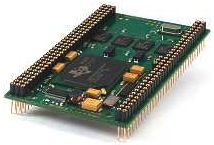
\includegraphics[width=\textwidth]{images/03_Realisierung/DSP6713}
                \caption{D.Module.C6713}
                \label{fig:D.Module.C6713}
        \end{subfigure}
        ~ %add desired spacing between images, e. g. ~, \quad, \qquad etc.
          %(or a blank line to force the subfigure onto a new line)
        \begin{subfigure}[b]{0.48\textwidth}
                \centering
                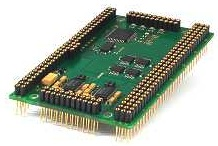
\includegraphics[width=\textwidth]{images/03_Realisierung/PCM3003}
                \caption{D.Module.PCM3003}
                \label{fig:D.Module.PCM3003}
        \end{subfigure}
        \caption{DSP-Flachbaugruppe D.Module.C6713 und A/D-Wandler D.Module.PCM3003}
        \label{fig:DSP_PCM3003}
\end{figure}
% ----------------------------------------- SUB-FIGURE -----------------------------------


Das D.Module.PCM3003 Modul ist ein Audiocodec, der speziell für Mehrkanal-Audio Signalverarbeitung sowie Mikrofonarrayverarbeitung designed wurde \cite[S. 1]{Manual_PCM3003}. \abb{PCM3003_blockdiagramm} zeigt alle Funktionsblöcke in einem Blockdiagramm. Der Codec verfügt über vier Stereo-ADC/DAC Module und kann so im Vierkanal-Stereo-Mode oder im Achtkanal-Mono-Mode betrieben werden. Da in dieser Arbeit acht Mikrofonsignale simultan verarbeitet werden sollen, wird der Achtkanal-Mono-Mode gewählt. Jedes der vier ADC/DAC-Module besitzt eine Auflösung von 16 bit und einen Delta-Sigma-Modulator 64. Ordnung. Alle ADC/DAC-Sektionen werden synchrone von einem einstellbaren Oszillator getaktet und können auf die im Audiobereich gängigen Abtastraten konfiguriert werden. Die Übertragung der Abtastwerte an den DSP erfolgt über zwei serielle Schnittstellen wobei jeweils zwei ADC/DAC-Stufen zu einer Schnittstelle führen. Alle notwendigen Synchronisationssignale werden von diesem Modul erzeugt, so dass es als Mastergerät fungiert.


\myFigure{real}                                                   % Figure tag (missing, real)
         {big}                                                       % Size (small,medium,big)
         {h!}                                                  % z.B. htbp
         {Blockdiagramm des D.SignT Moduls D.Module.PCM3003 (\vgl \cite[S. 1]{Manual_PCM3003})}    % Figure title
         {PCM3003_blockdiagramm}                                               % Figure label 
         {03_Realisierung/PCM3003_blockdiagramm} 



Das D.Module.C6713 Modul ist eine DSP Flachbaugruppe, dessen CPU\footnote{Central processing unit} der von \ti entwickelte TMS320C6713b aus der Prozessorreihe TMS320C6000 ist. Dieser DSP basiert 
auf einer Very Long Instruction Word Architektur mit einer Wortbreite von 256 bit und ist so in der Lange, bis zu acht 32-bit Befehle für jeweils einen der acht Funktionseinheiten innerhalb eines Taktschrittes zu verarbeiten \cite[S. 14]{Manual_dsp_datasheet}. Weiterhin kann der TMS320C6713b sowohl in Festkomma- als auch in Fließkomma-Arithmetik programmiert werden und unterstützt einen Prozessortakt von bis zu 300MHz wodurch eine Rechengeschwindigkeit von 1,8 GFLOPS\footnote{Giga-floating-point operations per second} erreicht werden kann. \abb{dsp_core_blockdiagramm} zeigt das Blockdiagramm mit der zur Verfügung stehenden Peripherie. Als Schnittstellen stehen unter anderem zwei Multi-channel-Buffered Serial Port (McBSP) und ein I2C Interface zur Verfügung, die mit Hilfe eines Enhanced Direct Memory Access (EDMA) Controller mit dem internen Speicher verknüpft sind. Die DSP-Flachbaugruppe bietet darüber hinaus noch folgende Funktionen:

\begin{itemize}
    \item 64 MB SDRAM\footnote{Synchronous Dynamic Random Access Memory} mit 100MHz Taktfrequenz
    \item 2MB Flash Speicher
    \item 256 kB Interner Speicher (für Programmcode sowie vom Programm benötigter Speicher)
    \item USB Schnittstelle zum PC inkl. JTAG\footnote{Joint Test Action Group} Emulator
    \item LED's sowie Taster zur Benutzerinteraktion
\end{itemize}


Als Programmierwerkzeug wird die von \ti entwickelte Softwarelösung \ccs verwendet.
Dieses Eclips-basierte Softwarepaket beinhaltet einen Sourcecode-Editor, eine Projektumgebung, eine Debug-Umgebung sowie die Möglichkeit Variable im laufenden Betrieb zu observieren und Speicherinhalte grafisch darzustellen. \ccs verfügt über einen C-Compiler, einen Assembler sowie einen Linker und wird in dieser Arbeit in Version 5 verwendet.


\myFigure{real}                                                   % Figure tag (missing, real)
         {max}                                                       % Size (small,medium,big)
         {h!}                                                  % z.B. htbp
         {Blockdiagramm des D.SignT DSP D.Module.C6713 (\vgl \cite[S. 1]{Manual_C6713})}    % Figure title
         {C6713_blockdiagramm}                                               % Figure label 
         {03_Realisierung/C6713_blockdiagramm} 



\myFigure{real}                                                   % Figure tag (missing, real)
         {max}                                                       % Size (small,medium,big)
         {h!}                                                  % z.B. htbp
         {Blockdiagramm der TMS320C6713b CPU (\vgl \cite[S. 13]{Manual_dsp_datasheet})}    % Figure title
         {dsp_core_blockdiagramm}                                               % Figure label 
         {03_Realisierung/dsp_core_blockdiagramm} 




% ****************************************************************************************
\subsection{Kommunikationsschnittstelle zwischen DSP und PCM3003}
\label{subsec:Kommunikationsschnittstelle_DSP_PCM3003}
% ****************************************************************************************
Als Kommunikationsschnittstelle zwischen DSP und PCM3003 dienen die vom DSP bereitgestellten McBSP. Der Datenaustausch findet so jeweils über zwei Datenleitungen statt, wobei eine die eingehenden und die andere die ausgehenden Daten enthält. Steuersignale wie Synchronisation und Taktung werden über eine separate Leitung übertragen. \abb{McBSP_blockdiagramm} illustriert das Funktionsblockdiagramm eines McBSP Moduls. Eine detaillierte Erklärung zu den Funktionen der einzelnen Pins und Register befindet sich in \cite{Manual_McBSP_Report}.
Die Übertragung der Daten in einem seriellen Datenstrom findet in einem speziellen Musterstatt wie in \tab{McBSP_Muster} dargestellt.


\myFigure{real}                                                   % Figure tag (missing, real)
         {small}                                                       % Size (small,medium,big)
         {h!}                                                  % z.B. htbp
         {McBSP Fubktionsblockdiagramm (\vgl \cite[S. 2]{Manual_McBSP_Report})}    % Figure title
         {McBSP_blockdiagramm}                                               % Figure label 
         {03_Realisierung/McBSP_blockdiagramm} 



Ein Muster dieser Art entsteht, da der PCM3003 die Ausgabedaten zweier ADC auf eine Datenleitung zusammenfasst (Multiplexing) und an den DSP versendet. Im Umkehrschluss findet eine Trennung der zusammengefassten Daten statt (Demultiplexing), wenn der DSP Daten an den PCM3003 überträgt. \abb{McBSP_reihenfolge} zeigt, in welcher Reihenfolge die Kanäle in die beiden Datenströme zusammengefasst werden \cite{Code_PCM3003Demo}. 

\begin{table}[h]
     \center
     \begin{tabular}{clc}
     \hline
          Codec & Kanal &  DSP-Kanal  \\
          \hline \hline
          1     & links      & 0      \\
          2     & links      & 2      \\
          1     & rechts     & 1      \\
          2     & rechts     & 3      \\
          3     & links      & 4      \\
          4     & links      & 6      \\
          3     & rechts     & 5      \\
          4     & rechts     & 7      \\
         \hline
     \end{tabular}
  \caption{McBSP Kanalzuordnung}
 \label{tab:McBSP_Muster}
 \end{table}




\myFigure{real}                                                   % Figure tag (missing, real)
         {big}                                                       % Size (small,medium,big)
         {h!}                                                  % z.B. htbp
         {Reihenfolge des Kanalmultilexing durch den McBSP}    % Figure title
         {McBSP_reihenfolge}                                               % Figure label 
         {03_Realisierung/McBSP_reihenfolge}


% ****************************************************************************************
\subsection{EDMA-Verfahren}
\label{subsec:EDMAVerfahren}
% ****************************************************************************************
Der herkömmliche Weg, Abtastwerte aus einem ADC-Register zu lesen, ist durch Verwendung einer Interrupt-getriggerten Funktion (ISR\footnote{Interrupt Service Routinen}). Dies bedeutet allerdings, dass der DSP im Intervall der Abtastfrequenz seine aktuelle Operation unterbrechen muss, um die ISR auszuführen. In Anbetracht eines echtzeitfähigen Systems, in dem alle Berechnungen innerhalb eines Signalblocks (besteht hier aus einer Anzahl von 256 Abtastwerten) erfolgen müssen sind Unterbrechungen solcher Art von großem Nachteil. 

Zur Vermeidung von Unterbrechungen ist es erforderlich, dass der Prozess der Datensammlung einem zusätzlichen Modul zugeteilt wird. Das System verwendet daher den EDMA-Controller zur Sammlung von Abtastwerten. Mit einer vorher definierten Blockgröße informiert der EDMA-Controller den DSP mit Hilfe eines Interrupt, wann ein Block bereit zur Datenverarbeitung ist. Des Interrupt-Intervall hängt nun von der Abtastfrequenz sowie der Blocklänge ab. Die Kommunikationsschritte zwischen DSP und EDMA-Controller lassen sich wie in \abb{EDMA_Interrupt} dargestellt chronologisch auflisten:

\begin{enumerate}
    \item Die Hauptroutine initialisiert alle nötigen EDMA-Register und startet diesen.
    \item Die Hauptroutine wartet auf den Interrupt vom EDMA-Contoller welcher signalisiert, dass ein Signalblock bereit zur Datenverarbeitung ist-
    \item Die Datenverarbeitung beginnt, sobald ein EDMA-Interrupt empfangen wurde.
    \item Nach Beenden der Datenverarbeitung wartet die Hauptroutine auf den nächsten EDMA-Interrupt.
\end{enumerate}


\myFigure{real}                                                   % Figure tag (missing, real)
         {big}                                                       % Size (small,medium,big)
         {h!}                                                  % z.B. htbp
         {Interrupthandling zwischen EDMA-Controller und der Hauptroutine}    % Figure title
         {EDMA_Interrupt}                                               % Figure label 
         {03_Realisierung/EDMA_Interrupt}



% ****************************************************************************************
\subsection{Ping-Pong-Speicherverfahren}
\label{subsec:PingPongSpeicherverfahren}
% ****************************************************************************************
Zur Vermeidung von Datenverlust während der Datenverarbeitung eines Signalblocks sowie die zur Schaffung einer Möglichkeit zur unkomplizierten Einstellung des Zeitverhalten der Datenverarbeitungsroutine wird im Folgenden ein Ping-Pong-Speicherverfahren (Doublebuffer) angewendet. Hierbei sind anstelle eines Speicherfeldes zwei Felder mit identischer Größe im Einsatz. Wie in \abb{ping_pong_verfahren} dargestellt, alterniert die Datenverarbeitung zwischen diesen beiden Speichern. Vorteil dieser Methode ist, dass während der Verarbeitung eines Datenblocks im Hintergrund (nebenläufig) der zweite Block mit neuen Daten beschrieben wird. So kommt es bei den kontinuerlich am Mikrofonarray eintreffenden Audiosignalen zu keinem Datenverlust. Weiterhin entsteht so eine definierter Zeitabschnitt, in dem der Algorithmus seine Berechnungen abgeschlossen haben muss. Die wesentlichen Schritte dieses Verfahrens lassen sich wie folgt auflisten:


\begin{enumerate}
    \item Der EDMA-Controller erhält Daten vom der PCM3003 und speichert sie im Ping-Speicher.
    \item Ist die Blockgrenze des Ping-Speichers erreicht, beginnt der EDMA-Controller seinen Speichervorgang auf dem Pong-Speicher, sendet einen Interrupt an den DSP und gibt somit den Ping-Speicher zur Verarbeitung frei.
    \item Ist die Blockgrenze des Pong-Speichers erreicht, wird dieser ebenfalls mit einem Interrupt zur Verarbeitung freigegeben und die Prozedur beginnt erneut.
\end{enumerate}
 
\myFigure{real}                                                   % Figure tag (missing, real)
         {Big}                                                       % Size (small,medium,big)
         {h!}                                                  % z.B. htbp
         {Ping-Pong-Verfahren der Hauptroutine (\vgl \cite[S. 35]{Master_Array_Pikora})}    % Figure title
         {ping_pong_verfahren}                                               % Figure label 
         {03_Realisierung/ping_pong_verfahren}



% ****************************************************************************************
\section{Algorithmische Umsetzung}
\label{sec:AlgorithmischeUmsetzung}
% ****************************************************************************************
Im folgenden Abschnitt soll nun gezeigt werden, auf welche Weise die Implementierung der einzelnen Systemfunktionen in der Programmiersprache C umgesetzt wurde. Im Vergleich zur in \Sec{sec:Simulation} beschriebenen Simulation in \matlab, die in Bezug auf Genauigkeit sowie Geschwindigkeit idealen Bedingungen unterliegt, besitzt der DSP diesbezüglich klare Einschränkungen, die zur Gewährleistung einer stabilen Programmfunktion beachtet werden müssen.

In Bezug auf den verwendbaren Zahlenbereich arbeitet \matlab standardmäßig mit doppelter Genauigkeit. In C entspricht das dem Variablentyp \code{double} mit einer Größe von 64 bit. Da der DSP in dieser Anwendung in Fließkommaarithmetik programmiert wird und lediglich einen internen Speicher von 256kB besitzt, erfolgt die Auflösung von Zahlen maximal mit dem 32 bit Datentyp \code{float}. Des weiteren gilt es, Kopiervorgänge von Feldinhalten weitestgehend zu vermeiden und die von C zur Verfügung gestellte Zeigerarithmetik auszunutzen. 


% ****************************************************************************************
\subsection{Aufbau des C-Projekts}
% ****************************************************************************************
Der Aufbau des C-Projekts ist in \scr{ProjektAufbau} dargestellt. Es beinhaltet drei C-Dateien, in denen die gesamte Funktionalität abgebildet ist. Die Datei \code{main.c}, enthält die Hauptroutine \code{main()} in welcher sich der Algorithmus zur Sprecherlokaliserung befindet. In der Datei \code{defines\_globales.c} befindet sich lediglich eine Funktion \code{init()}. Diese wird zu Beginn des Programms aufgerufen und initialisiert alle benötigten Konstanten. Sie Datei \code{functions.c} beinhaltet alle benötigten Funktionen zur Berechnung der Sprecherposition. Sie können aus \code{main.c} aufgerufen werden.

% **************************************************************
\pagebreak
% **************************************************************

\begin{lstlisting}[caption={Aufbau des C-Pojekts}, label=lst:ProjektAufbau,frame=htlrb, firstnumber=1]
    main.c
      |-- bios.h
      |-- setup.h
      |-- functions.h
      |-- defines_globales.h
    
    defines_globales.c
      |-- defines_globales.h
      |-- functions.h
      |-- DSPF_sp_bitrev_cplx.h
      
    functions.c
      |-- functions.h
      |-- defines_globales.h
      |-- DSPF_sp_cfftr2_dit.h
      |-- DSPF_sp_icfftr2_dif.h
      |-- DSPF_sp_bitrev_cplx.h
\end{lstlisting}




% ****************************************************************************************
\subsection{Headerdateien des Projekts}
\label{subsec:HeaderdateienDerProjekts}
% ****************************************************************************************
Zur bequemeren Einstellung der zur Verfügung stehenden Programmmodi wurde die Headerdatei \code{setup.h} erstellt. In ihr befinden sich die folgenden Makros zur Manipulation der Programmfunktion:


\paragraph{Auswahl des Programmmodus} Das Makro \code{C\_MODE\_ON} bestimmt, ob das Programm im C-Mode läuft und alle hardwarespezifischen Programmelemente ausblendet. Hierfür muss in der Datei \code{main.c} eine entsprechende Headerdatei gewählt werden, aus der der Algorithmus synthetisch erzeugte Abtastwerte entnehmen kann.

\paragraph{Debug-Modus} Das Makro \code{DEBUG\_MODE\_ON} schaltet den Debug-Modus ein, wodurch Debug-Nachrichten unter Verwendung der Funktion \code{printf()} auf die Konsole geschrieben werden. 

\paragraph{Überprüfung des Zeitverhaltens} Das Makro \code{PROFILE\_MODE\_ON} bewirkt, dass die Messung des Zeitverhaltens mit Hilfe der GPIO\footnote{General-purpose input/output} Ausgänge stattfinden kann. Zur zusätzlichen Echtzeitkontrolle kann das Makro \code{ADC\_LOOP\_THROUGH\_MODE\_ON} gesetzt werden, wodurch die Daten aus Kanal 1 des ADC direkt auf Kanal 1 des DAC kopiert wird.

\paragraph{Serielle Übertragung der Daten} Durch das Setzen des Makros \code{UART\_MODE\_ON} versendet der DSP nach jeder Berechnung einer gültigen Sprecherposition beiden Raumwinkel $\phi$ und $\theta$ mit Hilfe der UART\footnote{Universal Asynchronous Receiver Transmitter}-Schnittstelle.


\paragraph{Einschalten der Optimierung} Das Makro \code{HISTOGRAM\_MODE\_ON} bewirkt die Filterung des Ergebnisses mit Hilfe eines Histogramms. Die Einstellungen zur Histogrammlänge sowie der Schwelle befinden sich in der Datei \code{defines\_globales.h}.\newline

Weiterhin existiert die Headerdatei \code{defines\_globales.h} sowie \code{functions.h}. \code{defines\_globales.h} enthält alle vordefinierten Konstanten. Zur fehlerfreien Programmfunktion wird empfohlen, alle, außer die Werte in der Histogrammsektion, unverändert zu lassen. In der Datei \code{functions.h} befinden sich alle Funktionsprototypen, so dass durch Einbindung dieser Headerdatei in eine andere C-Datei auf alle Funktionen zugegriffen werden kann.

% ****************************************************************************************
\subsection{DSP Speicherbelegung}
\label{subsec:DSPSpeicherbelegung}
% ****************************************************************************************
Das DSP-Modul verfügt wie oben genannt über 256kB internen Speicher sowie über 2MB Flash Speicher, die für das Programm genutzt werden können. Es stehen 64MB SDRAM zur Verfügung, die im Vergleich zum internen Speicher nur mit einem Drittel der Geschwindigkeit operieren. Nach einem Test des Programms unter Verwendung dieses Speichers stellte sich heraus, dass sich dieser für den Echtzeitbetrieb als ungeeignet erweist.

Die Größen für den Stack-und Heapspeicher wurden, wie durch das Demoprogramm vorgegeben, beibehalten. Der Stack hat eine Größe von 1024 Byte und der Heap eine Größe von 4096 Byte.

Aufgrund der Verwendung von acht Mikrofonen und einer Blocklänge von 256 Abtastwerten nehmen die Felder, welche die Abtastwerte sowie die Kreuzkorrelationsfunktionen enthalten, den meisten Speicherplatz ein. Mit einer Gesamtgröße von ca. 147kB nehmen sie ca. 57\% des Gesamtspeichers ein.

Zur Verkleinerung der Zugriffszeiten auf Variable mit dem Datentyp \code{st\_complex} wurden diese mit dem Pragmabefehl \code{DATA\_ALIGN} nur auf gerade Adressen im Speicher abgelegt. Dies erhöht die Zugriffsgeschwindigkeit bei der Verwendung der FFT-Routine (\vgl \cite[S. 67]{Master_Array_Pikora}).

Zur Optimierung der Geschwindigkeit wurden alle Funktionen der Datei \code{functions.c} wie in \cite{Manual_TMS320C6000_opt} beschrieben, in der Stufe 5 vom Compiler optimiert. Zu beachten ist, dass sich solch eine Optimierung zu Lasten des verwendeten Speichers auswirkt.



% ****************************************************************************************
\subsection{Ablauf der Hauptroutine}
\label{subsec:AblaufDerHauptroutineg}
% ****************************************************************************************
\abb{main_ablaufdiagramm} zeigt den Ablauf der Hauptroutine \code{main()}, welche sich in der Datei \code{main.c} befindet. Als Grundlage dieser Datei diente das von D.SignT bereitgestellte Demoprogramm \code{pcm3003}, welches bereits die Nutzung des EDMA sowie die Ping-Pong-Speichertechnik für acht Kanäle beinhaltete. Die wesentlichen Bestandteile dieser Datei sind:


\begin{itemize}
    \item Initialisierung aller notwendigen Hardware
        \begin{itemize}
            \item DSP-Modul
            \item UART-Modul
            \item Zurücksetzen des PCM3003
            \item Konfiguration der beiden McBSP
            \item Konfiguration des EDMA-Controllers
        \end{itemize}
    \item Initialisierung aller Variablen und Methoden des Algorithmus
    \item Algorithmus zur Sprecherlokalisierung 
\end{itemize}

Wie in \abb{main_ablaufdiagramm} dargestellt, läuft die Routine in einer Endlosschleife und kann nur durch Abschalten des DSP beendet werden.


\myFigure{real}                                             % Figure tag (missing, real)
         {medium}                                              % Size (small,medium,big)
         {h!}                                                  % z.B. htbp
         {Ablaufdiagramm der Hauptroutine \code{main()}}       % Figure title
         {main_ablaufdiagramm}                                 % Figure label 
         {03_Realisierung/main_ablaufdiagramm}                 % Path to real figure




% ****************************************************************************************
\subsection{Methodenumsetzung}
\label{subsec:Methodenumsetzung}
% ****************************************************************************************
In diesem Abschnitt folgt eine detaillierte Beschreibung, auf welche Weise die benötigten Funktionalitätenin Funktionen der Programmiersprache C umgesetzt wurden. 




% ****************************************************************************************
\subsubsection{Energieberechnung}
% ****************************************************************************************
Die Berechnung der Blockenergie erfolgt als erster Schritt in der Hauptroutine. Das Ergebnis zeigt an, ob der aktuelle Signalblock als stimmhaftes Sprachsignal interpretiert wird oder nicht. Auf Grund der kleinen Abstände zwischen den Sensoren wird angenommen, dass sich die Energie von einem Mikrofon zum anderen kaum unterscheidet. Aus diesem Grund wird nur der Signalblock von Sensor 1 betrachtet. Erreicht der Energiewert die Blockenergieschwelle \code{ENERGIE\_LIMIT} wird dieser als gültig markiert und für die Berechnung der Sprecherposition verwendet.

%\begin{lstlisting}[caption={Berechnung der Blockenergie für einen Kanal}, label=lst:energie,frame=htlrb, firstnumber=1]
%  for ( i=0; i < int16_BufLen; i++ ) {
%    f_Dest += (float) (int16_Scr[i] * int16_Scr[i]);
%  }
%  
%  return ( f_Dest * INV_N_SAMPLES * CONVERT_INT16_TO_FLOAR );
%\end{lstlisting}




% ****************************************************************************************
\subsubsection{Einlesen eines Datenblocks}
% ****************************************************************************************
Aufgrund der Verarbeitung der Daten in Fließkommaarithmetik ist es notwending, die vom ADC gelieferten Festkommawerte in das Format \code{float} zu konvertieren. Da es sich hierbei um komplexwertige Signalverarbeitung handelt, findet die Speicherung in einer komplexen Struktur vom Typ \code{st\_compelx} statt. Des weiteren erfolge wie in \scr{copy2cmpxStr} dargestellt das Zero-Padding für die zweite Hälfte des komplexen Feldes.


% **************************************************************
\pagebreak
% **************************************************************

\begin{lstlisting}[caption={Einlesen eines Datenblocks vom ADC inkl. Zero-Padding}, label=lst:copy2cmpxStr,frame=htlrb, firstnumber=1]  
for ( i=0; i < int16_ScrLen; i++ ) {
    
    // copy source buffer to complex struct
    st_Dest[i].re = ( (float) int16_Scr[i] ) * CONVERT_INT16_TO_FLOAR;
    st_Dest[i].im = 0.0;
    
    // do zero-padding for second half of destination buffer
    st_Dest[i+int16_ScrLen].re = 0.0;
    st_Dest[i+int16_ScrLen].im = 0.0;
}
\end{lstlisting}


% ****************************************************************************************
%\subsubsection{Varianzberechnung}
% ****************************************************************************************

%\begin{lstlisting}[caption={Berechnung aller Varianz Elemente der Matrix $\mathbf{R}_{\phi,\theta}$}, label=lst:label,frame=htlrb, firstnumber=1]
%    // Calculate variance elements of R
%    for ( i=0; i < int16_NumOfMics; i++ ) {
%        // Reset variance element i
%        f_Dest[i] = 0;
%        for ( j=0; j < int16_BufLen; j++ ) {
%            f_Dest[i] += (st_Scr[i][j].re * st_Scr[i][j].re);
%        }
%        // Norm variance to buffer length
%        f_Dest[i] = f_Norm * f_Dest[i];
%    }
%\end{lstlisting}



% ****************************************************************************************
\subsubsection{Schnelle Kreuzkorrelation}
% ****************************************************************************************
Die Berechnung der Kreuzkorrelation wurde wie in \Sec{subsubsec:SchnelleKreuzkorrelatio} beschrieben über die Multiplikation der Signalspektren realisiert. Grundsätzlich müssen dafür auf Grund der Symmetrieeigenschaft 28 Kreuzkorrelationsfunktionen berechnet werden. Wie in \abb{fcc_ablaufdiagramm} dargestellt erfolgt dies über sukzessive Berechnung und konjugiertkomplexe Multiplikation der Spektren mit anschließender Realteilbildung.



\myFigure{real}                                             % Figure tag (missing, real)
         {small}                                              % Size (small,medium,big)
         {h!}                                                  % z.B. htbp
         {Ablaufdiagramm der Kreuzkorrelationsroutine}       % Figure title
         {fcc_ablaufdiagramm}                                 % Figure label 
         {03_Realisierung/fcc_ablaufdiagramm}                 % Path to real figure




Zur Berechnung des Kreuzleistungsdichtespektrums über die konjugiert komplexe Multiplikation wurde folgender Zusammenhang genutzt:

\begin{equation}\label{eq:kplxKonjMul}
    (\mathrm{Re}_{1} + \im \, \mathrm{Im}_{1}) \cdot (\mathrm{Re}_{2} + \im \, \mathrm{Im}_{2})^* = \mathrm{Re}_{1}\mathrm{Re}_{2} + \mathrm{Im}_{1}\mathrm{Im}_{2} + \im \, (\mathrm{Im}_{1}\mathrm{Re}_{2} - \mathrm{Re}_{1}\mathrm{Im}_{2})
\end{equation}

Des Weiteren erfolgte die Ermittlung der Signalspektren über die von \ti zur Verfügung gestellten Softwarebibliothek TMS320C67x DSP Library\cite{Manual_dsp_lib}. Diese enthält spezielle für diesen Prozessortyp hochoptimierte Assemblerroutinen. Zur Transformation in den Frequenzbereich wurde die Funktion \code{DSPF\_sp\_cfftr2\_dit()} \cite[S. 4-13]{Manual_dsp_lib} verwendet. Zur Rücktransformation in den Zeitbereich kam die Funktion \code{DSPF\_sp\_icfftr2\_dif()} \cite[S. 4-34]{Manual_dsp_lib} zum Einsatz. Diese beiden Funktionen führen ihre Berechnungen unter Angabe eines Datenfeldes, einer Feldlänge sowie den Twiddlefaktoren durch. 
Die Daten müssen in komplexer Form vorliegen wobei Realanteil und Imaginäranteil hintereinander angeordnet sind: $\mathrm{Re}(x_0), \mathrm{Im}(x_0), \mathrm{Re}(x_1), \mathrm{Im}(x_1), \dots, \mathrm{Re}(x_{N-1}), \mathrm{Im}(x_{N-1})$. Zu beachten ist, dass das Datenfeld für Eingangs- sowie Ausgangswerte genutzt wird und die Eingangsdaten somit durch die Ausgangsdaten überschrieben werden. Da die Twiddle-Faktoren $\underline{W}^k_N$ nur von der FFT-Länge abhängig sind, können diese in der Initialisierungsphase erstellt werden. Sie sind gegeben durch(\vgl \cite[S. 2]{Slide_Sauvagerd_FFT}): 
\begin{equation}
    \underline{W}^k_N = e^{-\im\frac{2 \pi k}{N}} = \cos{\left(\delta \cdot k\right)} - \im \, \sin{\left(\delta \cdot k\right)} \eqspace \text{mit} \eqspace  \delta = \frac{2 \pi}{N}     
\end{equation}
\scr{twiddleFaktoren} zeigt die Erstellung dieser Faktoren innerhalb einer Schleife in der \code{init()}-Funktion. Des Weiteren findet hier unter Verwendung der Funktionen \code{digitrev\_index()} und \code{DSPF\_sp\_bitrev\_cplx()} die Anpassung der Twiddlefaktoren in die bitweise umsortierte Form für die FFT statt.

% **************************************************************
\pagebreak
% **************************************************************

\begin{lstlisting}[caption={Erstellung der Twiddlefaktoren innhalb einer Schleife in der \code{init()}-Funktion.}, label=lst:twiddleFaktoren,frame=htlrb, firstnumber=1]
  for( i = 0; i < N_CORRELATION/RADIX; i++ ) {
    W[i].re = (float)  cos(DELTA*i);   // real pos component of W
    W[i].im = (float) -sin(DELTA*i);   // neg imag component of W
  }
  // produces index for bitrev() W
  digitrev_index( iTwid, N_CORRELATION/RADIX, RADIX );  
  DSPF_sp_bitrev_cplx( (double*) W , iTwid, N_CORRELATION/RADIX );
\end{lstlisting}



\scr{fcc} zeigt den Aufbau der Korrelationsroutine. Hier werden zunächst alle acht Zeitsignale in den Frequenzbereich transformiert. Anschließend erfolgt die Berechnung des Kreuzleistungsdichtespektrums unter Verwendung der Funktion \code{CmplxConjMul()} sowie die Rücktransformation in den Zeitbereich mit Hilfe von \code{DSPF\_sp\_icfftr2\_dif()}. Im Hinblick auf einen späteren Betrieb in Echtzeit ist es sinnvoll, sparsam mit dem zur Verfügung stehenden Speicher umzugehen, da die Länge eines EDMA-Rahmens unter Umständen vergrößert werden muss. Aus dieseM Grund wird darauf verzichtet, jede der 28 Kreuzkorrelationsfunktionen in voller Länge  abzuspeichern (512 Abtastwerte). Statt dessen exsistiert lediglich ein zentrales Array (\code{st\_Buf.f\_CmplxSigBufXY}) in dem genau ein KKF abgelegt werden kann. Wie in \scr{fcc} dargestellt, wird der KKF, unter Berücksichtigung der maximalen Korrelationsdauer (siehe \Sec{subsubsec:Signalblocklaenge}) ein Datenblock der Länge $K_{New} = 2K_{max} + 1$ entnommen und in einem separaten Feld abgelegt. Diese Vorgehen ist möglich, da wie bereits erwähnt, lediglich auf $K_{New}$ Abtastwerte im Intervall $-K_{max} \leq n \leq K_{max}$ zugegriffen wird. Im Vergleich zur herkömmlichen Speicherung aller Abtastwerte, erzielt dieses Vorgehen eine Speicherersparnis von 53,6 kB (entspricht ca. 30\% des Gesamtspeichers).

% **************************************************************
\pagebreak
% **************************************************************

\begin{lstlisting}[caption={Berechnung der Kreuzkorrelationsfunktionen}, label=lst:fcc,frame=htlrb, firstnumber=1]
  // Calculate all FFT's in place
  for ( i=0; i < int16_NumOfMics; i++ ) {
    DSPF_sp_cfftr2_dit( (float*) st_Scr[i], (float*) W, int16_BufLen );
  }
  // Calculate Cross-Correlation-Functions in place
  n = 0;
  for ( i=0; i < (int16_NumOfMics-1); i++ ) {			// Row
    for ( j=(i+1); j < int16_NumOfMics; j++ ) {		// Column  
      CmplxConjMul( st_Scr[i], st_Scr[j], st_Helper, int16_BufLen );
      DSPF_sp_icfftr2_dif( (float*) st_Helper, (float*) W, int16_BufLen );
      // Set Zero-Element
      st_Dest[n][((MAX_DELAY-1)/2)] = st_Helper[0].re * INV_N_CORRELATION;
      // Store required date block of n-th CCF (only real-component)
      for( k=0; k < (MAX_DELAY-1)/2; k++) {
        st_Dest[n][k] = st_Helper[k + int16_BufLen - (MAX_DELAY-1)/2].re * INV_N_CORRELATION;
        st_Dest[n][k+ ((MAX_DELAY+1)/2)] = st_Helper[k+1].re * INV_N_CORRELATION;
      }
      n++;
    }
  }
\end{lstlisting}


% ****************************************************************************************
\subsubsection{Mehrkanal-Kreuzkorrelationskoeffizient}
% ****************************************************************************************
Zur Berechnung des Mehrkanal-Kreuzkorrelationskoeffizienten werden folgende Schritte durchgeführt:

\begin{enumerate}
    \item Berechnung des Suchbereichs $C_{\phi,\theta}$.
    \item Berechnung der Verzögerungen zu den theoretischen Raumwinkeln $\phi$ und $\theta$.
    \item Erstellung der räumlichen Korrelationsmatrix $R_{\phi,\theta}$.
    \item Berechnung der Determinanten $\det\left[R_{\phi,\theta}\right]$.
    \item Wiederholung bei Punkt 1 bis minimaler Suchbereich $C_{\phi,\theta_{min}}$ erreicht ist. 
\end{enumerate}


%\abb{mccc_ablaufdiagramm} zeigt das Ablaufdiagramm des Berechnungsalgorithmus. 
Die gesamte Berechnung wurde in die Funktion \code{SearchAndFind()} ausgelagert, die \ua einen Zeiger auf die Struktur erhält, in der Kreuzkorrelationsfunktionen enthalten sind. Hier wird zunächst wie in \Sec{subsubsec:Suchgeschwindigkeit} beschrieben der Suchbereich $C_{\phi,\theta}$ zur optimierten Suche berechnet. Anschließend erfolgen die Berechnung der theoretischen Verzögerungen und die Erstellung der räumlichen Korrelationsmatrix $R_{\phi,\theta}$ sowie die Berechnung von dessen Determinante. Dieser Vorgang wird solange wiederholt, bis alle Richtungen im Suchbereich durchlaufen wurden. Anschließend erfolgt die Verkleinerung des Suchbereiches und der Vorgang beginnt erneut. Erreicht der Suchbereich sein Minimum, können die gefundenen Raumwinkel als globales Minimum angesehen werden und der Algorithmus endet.

Zur Berechnung der theoretischen Laufzeitunterschiede wurde die Funktion \code{UCAFunctionTauRound} verwendet. Zur Erstellung der räumlichen Korrelationsmatrix dient die Funktion \code{Create\_R()}, die mit Hilfe der theoretischen Verzögerungen den 28 Kreuzkorrelationsfunktionen 64 Werte entnimmt, um die Matrix $R_{\phi,\theta}$ zu bilden.

Zur Berechnung der Determinante existiert die Funktion \code{CalcDetNxN()}. Determinanten von Matrizen bis zu einer Größe von $3 \times 3$ sind durch klare Rechenvorschriften zu ermitteln. Für Determinanten höherer Ordnung müssen spezielle Verfahren wie das gaußsche Eliminationsverfahren, die Leibniz-Formel oder der Laplace'sche Entwicklungssatz verwendet werden. Auf Grund eines erhöhten Rechenaufwands der letzten beiden Methoden wird im Folgenden das gaußsche Eliminationsverfahren implementiert, das in der Lage ist, eine $N \times N$ Determinate zu berechnen. Dazu muss die Matrix $\mathbf{A}$, gegeben durch:
\begin{equation}
\mathbf{A} = 
    \begin{bmatrix}
        a_{1,1} & a_{1,2} & \dots  & a_{1,N} \\
        a_{2,1} & a_{2,2} & \dots  & a_{2,N} \\
        \vdots  & \vdots  & \ddots & \vdots  \\
        a_{N,1} & a_{N,2} & \dots  & a_{N,N}
    \end{bmatrix}
\end{equation}

unter Verwendung elementarer Zeilenumformungen in die obere Dreiecksform gebracht werden. Dies bedeutet, alle Elemente unterhalb der Hauptdiagonalen müssen den Wert Null betragen. Die Matrix $\mathbf{A}$ mit den veränderten Koeffizienten $b_{i,j}$ ist somit gegeben durch:

\begin{equation}
\mathbf{A} = 
    \begin{bmatrix}
        b_{1,1} & b_{1,2} & \dots  & b_{1,N} \\
        0       & a_{2,2} & \dots  & b_{2,N} \\
        \vdots  & \vdots  & \ddots & \vdots  \\
        0       & 0       & \dots  & b_{N,N}
    \end{bmatrix}
\end{equation}

Die Determinante kann nun als Produkt der Elemente auf der Hauptdiagonalen wie folgt ermittelt werden:

\begin{align}
    \det(\mathbf{A}) & = (-1)^r \cdot b_{1,1} \cdot b_{2,2} \cdot \dots \cdot b_{N,N} \\
                     & = (-1)^r \cdot \prod_{i=1}^{N} b_{i,i}
\end{align}

Der Parameter $r$ beschreibt dabei die Anzahl der durchgeführten Zeilenvertauschungen. 




%\myFigure{missing}                                             % Figure tag (missing, real)
%         {medium}                                              % Size (small,medium,big)
%         {h!}                                                  % z.B. htbp
%         {Ablaufdiagramm zur Berechnung des Mehrkanal-Kreuzkorrelationskoeffizienten}       % Figure title
%         {mccc_ablaufdiagramm}                                 % Figure label 
%         {03_Realisierung/mccc_ablaufdiagramm}                 % Path to real figure




    





% ****************************************************************************************
%\subsubsection{Optimiertes Suchverfahren}
% ****************************************************************************************




% ****************************************************************************************
\subsubsection{Histogrammoptimierung}
% ****************************************************************************************
\scr{histogramm} zeigt einen Ausschnitt der Histogrammerstellung für den Raumwinkel $\phi$. Die Erstellung des Histogramms erfolgt stets über den gesamten Ring-Speicher wobei nur gültige Werte (Werte größer als Konstante \code{INDEX\_INVALID}) entnommen werden. Um Rechenzeit einzusparen, erfolgt die Suche des Maximums bereits bei der Histogrammerstellung. Dazu wird der aktuelle Wert mit dem vorherigen verglichen. Ist der aktuelle Wert höher, wird dieser als neues Maximum markiert und dessen Index sowie Wert abgespeichert. Das identische Verfahren erfolgt im Anschluss für den zweiten Raumwimkel $\theta$. Erreicht der Maximalwert des Histogramms die Histogrammschwelle \code{int16\_HistogramThreshold}, wird dieser als gültiger Histogrammschätzwert markiert und kann ausgegeben werden.


\begin{lstlisting}[caption={Histogrammerstellung für den Raumwinkel $\phi$}, label=lst:histogramm,frame=htlrb, firstnumber=1]
  // Loop over entire histogram-ring-buffer
  for ( i=0; i < N_HISTOGRAM; i++ ) {

  // Check angle for validation (voiced)
  if ( int16_HistRingBuf[PHI][i] > INDEX_INVALID ) {

    // Increment histogram value by one
    st_Phi->int16_Hist[ int16_HistRingBuf[PHI][i] ]++;

    // Check maximum / store value and index
    if ( st_Phi->int16_Hist[ int16_HistRingBuf[PHI][i] ] > st_Phi->int16_HistEstVal ) {
       st_Phi->int16_HistEstVal = st_Phi->int16_Hist[ int16_HistRingBuf[PHI][i] ];
       st_Phi->int16_HistEstIdx = int16_HistRingBuf[PHI][i];
    }

    // Increment histogram counter
    PhiHistCnt++;
  }
\end{lstlisting}





% ****************************************************************************************
\subsubsection{Datenversand über RS232-Schnittstelle}
% ****************************************************************************************
Das Versenden der Schätzergebnisse erfolgt unter Verwendung der UART-Schnittstelle des DSP. Als Grundlage hierfür dient die zur Verfügung gestellte Funktion \code{send\_string()}. Diese erwartet einen Zeiger auf ein \code{char}-Array, in dem die zu sendenden Daten im ASCII\footnote{American Standard Code for Information Interchange}-Format enthalten sind. Da die gesamte Signalverarbeitung im Format \code{float} stattfindet,  muss hier zunächst eine Typ-Konvertierung durchgeführt werden. Als Grundlage hierfür steht die Funktion \code{stoa()} zur Verfügung. Diese ist in der Lage, eine Zahl im Format \code{short} in das benötigte ASCII Format zu bringen und einen Zeiger auf das ASCII Zeichen enthaltende \code{char}-Array zurückzugeben. Auf Grund der Ausgabe der Raumwinkel in Radiant wird die maximale Anzahl von Nachkommastellen auf vier begrenzt. Die Umformung vom Typ \code{float} in Typ \code{short} erfolgt durch Multiplikation mit dem Faktor $10^3$. Diese Operation verschiebt das Komma um drei Stellen nach rechts, so dass aus der Zahl 1,2345 die Zahl 1234,6 entsteht. Wie in \scr{float2Short} dargestellt, ergibt sich nach einer anschließenden cast-Operation der gewünscht Wert im Datentyp \code{short}. 


\begin{lstlisting}[caption={Konvertierung vom Datentyp \code{float} in Typ \code{short} mit 3 Nachkommastellen.}, label=lst:float2Short,frame=htlrb, firstnumber=1]
    int16_angle = (short) (1000 * f_angle)
\end{lstlisting}

%Zur Typ-Konvertierung stand die Funktion \code{Short2ASCII} zur Verfügung 
Da in dieser Anwendung zwei Winkelergebnisse versendet werden müssen, wird die \og Methode in die Funktion \code{Short2ASCII()} erweitert, so dass sich das in \abb{UART_Protokoll} dargestellte Kommunikationsprotokoll ergibt. Jeder Winkel kann somit in einem 6Byte langen \code{char}-Array abgebildet werden. Vor jedem Winkelwert wird ein entsprechender Winkel-
Identifizierer gesendet. Dieser zeigt an, ob es sich um den Raumwinkel $\phi$ oder $\theta$ handelt. Anschließend erfolgt das Senden des Wertes und dessen Vorzeichen. Hierbei ist wichtig, dass das Vorzeichen als letztes Zeichen gesendet wird, da es die Dekodierung der Zeichenkette auf Seiten des Empfängers enorm vereinfacht.



\myFigure{real}                                             % Figure tag (missing, real)
         {Big}                                              % Size (small,medium,big)
         {h!}                                                  % z.B. htbp
         {Zusammensetzung des Kommunikationsprotokolls zur Übertragung der Winkel unter Verwendung der UART-Schnittstelle.}       % Figure title
         {UART_Protokoll}                                 % Figure label 
         {03_Realisierung/UART_Protokoll}                 % Path to real figure




% ****************************************************************************************
\subsection{Displaycomponente des Systems}
\label{subsec:DisplaycomponenteDesSystems}
% ****************************************************************************************
Zur visuellen Ausgabe der ermittelten Raumwinkel wird im Folgenden eine graphische Benutzeroberfläche in der Programmiersprache Java entwickelt. Wie in \abb{gui} dargestellt, beinhaltet diese folgende Komponenten:

\begin{itemize}
    \item Data-LED zur Anzeige des Datenempfangs
    \item Dezimalanzeige des aktuellen Raumwinkels $\phi$ und $\theta$
    \item Prolardiagramm zur Anzeige des aktuellen Raumwinkels $\phi$ und $\theta$
    \item Bereich für Benutzerinteraktion
        \begin{itemize}
            \item Suchen nach sowie verbinden zu seriellen Schnittstellen
            \item Abspielen von Audiodateien (männlicher u. weiblicher Sprecher)
            \item Speichern von Ergebnisdaten im MAT-Format
            \item Einstellung des Formats (Radiant, Grad) der Dezimalzahlen für $\phi$ und $\theta$
            \item Einstellung theoretischer Winkel zur Namensgebung der MAT-Datei
        \end{itemize}
    \item Log und Debug Ausgabefenster
\end{itemize}


Zur übersichtlichen Organisation sowie zur robusten Kommunikation zwischen den einzelnen Klassen wird ein Model-View-Controller Konzept entworfen. Des Weiteren benötigt die Software einen Zustandsautomaten zum fehlerfreien Empfangen sowie zur robusten Dekodierung der Raumwinkel.



\myFigure{real}                                             % Figure tag (missing, real)
         {big}                                              % Size (small,medium,big,Big,max)
         {h!}                                                  % z.B. htbp
         {Graphische Benutzeroberfläche zur anschaulichen Darstellung der Winkelverläufe}       % Figure title
         {gui}                                 % Figure label 
         {03_Realisierung/gui}


% ****************************************************************************************
\subsubsection{Model-View-Controller}
% ****************************************************************************************
Die gesamte Software-Architektur richtet sich nach dem Model-View-Controller Konzept wie in \abb{gui_mvc} dargestellt. Hierbei existiert die Klasse \code{AppController}, die als oberste Controller-Klasse fungiert und somit die Kommunikation zwischen Model und View herstellt und überwacht. Als Model-Komponente wurden folgende Klassen implementiert:

\begin{itemize}
    \item \code{AudioHandler} - Dient zum Abspielen von Audiodaten über die integrierte Soundkarte
    \item \code{MatlabIOHandler} - Dient zum Speicherung der Raumwinkel in einem auf die Anwendung angepasstem Format.
    \item \code{SerialHandler} - Dient zur Kommunikation mit der seriellen Peripherie (Scan, Connect, Disconnect, \dots).
       \begin{itemize}
            \item \code{SerialValueHandler} - Wird von der Klasse \code{SerialHandler} instanziiert und implementiert den Zustandsautomaten zum Empfang und zur Dekodierung der Zeichenketten.
       \end{itemize}
\end{itemize}


Die View-Komponente besteht aus folgenden Klassen:

\begin{itemize}
    \item \code{ViewHandler} - Implementiert alle Methoden zur Erstellung der graphischen Benutzeroberfläche. Diese basieren auf dem von Java zur Verfügung gestellten \code{Swing/AWT}-Framework. Des Weiteren instanziiert diese Klasse zwei Objekte der Klasse \code{DiagramHandler} zur Erstellung der beiden Polardiagramme. Mir dem Aufruf der Methode \code{DiagramHandler.setAnglePointer()} kann dem Winkelzeiger der jeweilige Wert des Raumwinkels zugewiesen werden.
        \begin{itemize}
            \item \code{DiagramHandler} - Wird aus der Klasse \code{ViewHandler} instanziiert und implementiert alle Methoden zur Manipulation der Polardiagramme
            \item \code{DataLedHandler} - Wird aus der Klasse \code{ViewHandler} instanziiert und implementiert alle Methoden zum Setzen der Data-LED. Diese zeigt an, wann Daten über die UART-Schnittstelle empfangen werden.
        \end{itemize}
\end{itemize}


\myFigure{real}                                             % Figure tag (missing, real)
         {big}                                              % Size (small,medium,big,Big,max)
         {h!}                                                  % z.B. htbp
         {Model-View-Controller Konzept der graphischen Benutzeroberfläche. Die durchgezogenen Linien symbolisieren eine direkte Verbindung. Linien in gestrichelter Darstellung bedeuten die Kommunikation über einen indirekten Weg mit Hilfe des Entwurfsmusters "`Beobachter"'.}       % Figure title
         {gui_mvc}                                 % Figure label 
         {03_Realisierung/gui_mvc}



Wie in \abb{gui_mvc} illustriert existieren direkte unidirektionale\footnote{Kommunikation nur in eine Richtung} Kommunikationswege (duchgezogene Linien) sowie indirekte unidirektionale Kommunikationswege (gestrichelte Linie). Das bedeutet, die Kommunikation findet unter Verwendung von RMI\footnote{Remote Method Invocation} nur vom Controller in Richtung Model und View statt. Um den Controller darüber informieren zu können ,dass neue Daten zur Anzeige in der View-Kompomnennte zur Verfügung stehen, muss eine Kommunikationsmöglichkeit in die andere Richtung vorliegen. Um auf rechenintensive Polling-Methoden zu verzichten, bei denen der Controller permanent in einer Schleife auf ein Ready-Flag im Model prüfen muss, wird das Beobachter-Muster (observer pattern) implementiert. Dabei existiert ein Beobachter (in diesem Fall die Controller-Klasse) und ein Veröffentlicher (in diesem Fall die Model-Klasse). Die Controller-Klasse registriert sich zunächst bei der Model-Klasse als Beobachter. Liegen Daten zur Abholung bereit, wird diese Information umgehend an alle Beobachter veröffentlicht, so dass diese entsprechend ihrer internen Logik reagieren können. In diesem Fall werden die Ergebnisse erneut unter Verwendung von RMI in der Model-Klasse abgeholt. Diese Technik ermöglicht, dass der Controller-Klasse während des Empfang und der Dekodierung der Zeichenketten Zeit für andere Algorithmusschritte zur Verfügung stehen.




% ****************************************************************************************
\subsubsection{Zustandsautomat}
% ****************************************************************************************
\abb{gui_stateMachine} zeigt den Ablauf des Zustandsautomaten zum Empfangen und zur Dekodierung der vom DSP gesendeten Zeichenketten. Werden keine Daten empfangen befindet sich der Automat im Zustand \code{IDLE}. Sobald serielle Daten zum Empfang vorliegen, wechselt er in den Zustand \code{CHECK}, empfängt die Daten Byteweise und prüft jedes Byte auf einen der beiden Winkelidentifizierer \code{p} oder \code{t}. Wird eines der beiden Prüfzeichen (Identifizierer) empfangen, begibt sich der Automat in den Zustand \code{RECEIVE}, in dem er nun fünf weitere Zeichen empfängt (vier Ziffern + Vorzeichen). Empfängt der Automat innerhalb der fünf Ziffern ein ungültiges Zeichen, wird dieser Winkel verworfen und der Zustand wechselt erneut in \code{CHECK}. Empfängt der Automat alle Ziffern korrekt, werden diese nach dem in \abb{schema_dekodierung} dargestellten Schema dekodiert und der Zustand wechselt erneut in \code{CHECK}. Dieser Vorgang wiederholt sich so lange, bis keine Daten zum Empfang zur Verfügung stehen. Der Automat wechselt dann in den Zustand \code{IDEL} und wartet auf neue Daten.



\myFigure{real}                                             % Figure tag (missing, real)
         {Big}                                              % Size (small,medium,big,Big,max)
         {h!}                                                  % z.B. htbp
         {Darstellung des Zustandsautomaten der Klasse\\\code{SerialValueHandler}.}       % Figure title
         {gui_stateMachine}                                 % Figure label 
         {03_Realisierung/gui_stateMachine}


\myFigure{real}                                             % Figure tag (missing, real)
         {medium}                                              % Size (small,medium,big,Big,max)
         {h!}                                                  % z.B. htbp
         {Schema zur Dekodierung eines Zeichenketten-Frame}       % Figure title
         {schema_dekodierung}                                 % Figure label 
         {03_Realisierung/schema_dekodierung}



% ****************************************************************************************
%\subsubsection{Abspielen von Audiodaten}
% ****************************************************************************************


    

% ****************************************************************************************
\subsubsection{Export der Ergebnisse im MAT-Format}
% ****************************************************************************************
Zum Export der gespeicherten Raumwinkel im MAT-Format wird das Framework \code{jMatIO}\cite{web_jMatIO} verwendet. Das Framework unterstützt den Export von Daten in folgenden \matlab Formaten:

\begin{itemize}
    \item Double array 
    \item UInt8, Int8 array 
    \item UInt64, Int64 array 
    \item Char array 
    \item Structure 
    \item Cell array 
    \item Sparase array
\end{itemize}


\scr{saveMATFile} zeigt eine Methode der Klasse \code{MatIOHnadler}. Diese implementiert das Erstellen der entsprechenden \matlab Felder im den in Java gespeicherten Ergebniswerten. Dank der komfortablen API des \code{jMatIO}-Frameworks lässt sich dies durch simple Funktionsaufrufe realisieren. So lassen sich ebenfalls Zusatzinformationen wie einen Zeitstempel, der Sprechertyp sowie die theoretisch eingestellten Raumwinkel speichern um später die Ausgabe in \matlab weitestgehend zu automatisieren.

% **************************************************************
\pagebreak
% *************************************************************

\begin{lstlisting}[caption={Java-Funktion zum Export von Ergebniswerten in im MAT-Format}, label=lst:saveMATFile,frame=htlrb, firstnumber=1, language=java]
  public void createFile(){
    this.valueList.add( new MLChar( "created", simpleDateFormat.format( System.currentTimeMillis() ) ) );
    this.valueList.add( new MLChar( "audioType", this.audioType.toString() ) );
    this.valueList.add( new MLDouble( "anglesSetUp", this.angleSetUp, this.angleSetUp.length) );
    this.valueList.add( new MLDouble( "phi", phiValues.toArray(new Double[phiValues.size()]), phiValues.size()) );
    this.valueList.add( new MLDouble( "theta", thetaValues.toArray(new Double[thetaValues.size()]), thetaValues.size()) );

    try {
      new MatFileWriter(  this.filepath +
                          this.fileSeparetor +
                          this.fileName +
                          ".mat", valueList );
    } catch (IOException e) {
      e.printStackTrace();
    }
    this.phiValues.clear();
    this.thetaValues.clear();	
  }
\end{lstlisting}







